% This is samplepaper.tex, a sample chapter demonstrating the
% LLNCS macro package for Springer Computer Science proceedings;
% Version 2.20 of 2017/10/04
%
\documentclass[free]{flammie}
%
\usepackage{graphicx}
% Used for displaying a sample figure. If possible, figure files should
% be included in EPS format.
%
% If you use the hyperref package, please uncomment the following line
% to display URLs in blue roman font according to Springer's eBook style:
% \renewcommand\UrlFont{\color{blue}\rmfamily}
\usepackage{booktabs}

\begin{document}
%
\title{Building language technology infrastructures to support a collaborative approach to language resource building}%---a survey of state-of-the-art in Uralic morphographemics and NLP}
%
%\titlerunning{Building language technology infrastructures}
% If the paper title is too long for the running head, you can set
% an abbreviated paper title here
%
\newcommand{\orcidID}[1]{$^{[#1]}$}

\author{Tommi A Pirinen\orcidID{0000-0003-1207-5395} \\
UiT-Norgga árktalaš universitehta \\
\url{firstname.lastname@uit.no}
\and
Francis M. Tyers\orcidID{0000-0001-6108-2220} \\
Indiana\\
\url{ftyers@iu.edu}
}
%
%\authorrunning{T.A Pirinen, F.M. Tyers}
% First names are abbreviated in the running head.

% If there are more than two authors, 'et al.' is used.
%
%\institute{UiT Norgga árktalaš universitehta\\
%\email{firstname.lastname@uit.no}\\
%\url{https://uit.no} \and
%Indiana \\
%\email{ftyers@iu.edu}
%}
%
\maketitle              % typeset the header of the contribution
%
\newcommand{\keywords}[1]{Keywords: \textit{#1}}
\begin{abstract}
Digital infrastructures are a vital part of support for providing a research framework and platform in engineering their digital lexicography and grammars and deploying the to end-users as real NLP software products.
In this article we review the usage of two popular free/libre open source infrastructures and give our view on best current practices from few decades of experiences.
We find that infrastructures can turn work in digital lexicography and grammars into viable end-user products like machine translators, spell checkers and correctors and so forth.
\keywords{NLP infrastructures \and Citizen science \and Uralic languages.}
\end{abstract}
%
%
%
\section{Introduction} \label{sec:intro}

Work in digital humanities, particularly like of digital lexicography, is a very front and central concept in building for language technologies and digital cultures for minority and under-resourced languages.
In these contexts, it is common to have very limited access to language experts that are highly necessary for building of the resources necessary, we talk about \textit{citizen science} and \textit{crowd-sourcing}.
For this reason, the role of digital infrastructures for building of the natural language processing systems becomes very central.
An ideal digital infrastructure makes it easy for a language expert, activist or other contributor with limited technical skills or resources to work with involved technically complex systems, to contribute their expertise with their native language skills.
In this article we make an overview of some infrastructures that enable contributing native language skills and describe some recent developments in the field of software engineering that have enabled us to improve our infrastructures so we also lay out a desiderata of a kinds for all sorts of language technology infrastructures.

In this article we use as a case study two infra-structures we have helped to build, that are also central to Uralic natural language processing: GiellaLT\footnote{\url{https://github.com/giellalt}} and Apertium\footnote{\url{https://github.com/Apertium}}, but we also cast an eyesight towards other kinds of popular infrastructures.

The article is organised in following sections: First we describe some background for the system in section~\ref{sec:background}.
Then we describe and compare different infrastructures and their features in section~\ref{sec:unfra}.
We discuss the system in section~\ref{sec:discussion}.

\section{Background} \label{sec:background}

The work on computational lexicography, specifically for finite-state language models and Uralic languages has been carried on for almost 40 years now.
Some of the technologies and systems underneath remain largely unchanged, for example Finite-State morphology~\cite{beesley2003finite} methods have been used in similar form ever since the beginning.
On the other end, the software engineering and computational infrastructures typically have life-cycle of not more than 10 years.
The role of infrastructure to support language scientists and contributors is in many cases to reduce the impact of changes of such computational systems to provide smooth continuity for the development of the actual dictionary data etc.
The scientists and language experts contributing words and grammars are usually not interested in differences of, e.g. RCS, CVS, SVN and git as version control system, while the infrastructures have been dragged through these all in the past decades---and conversely, the engineers who build the infrastructures may be very interested in such underlying technologies.
The linguistic and NLP software is built on lexical data and grammars, this includes software like:
\textit{machine translation}, \textit{spell-checking and correction}, \textit{grammar checking}, \textit{text-to-speech} and so forth.
The main point of a good infrastructure is that the lexical data can be contributed once and used for all applications alike.
In figure~\ref{fig:infra} there is a diagrammatic representation of ideal work-flow between various stakeholders of NLP software.

\begin{figure}
    \centering
    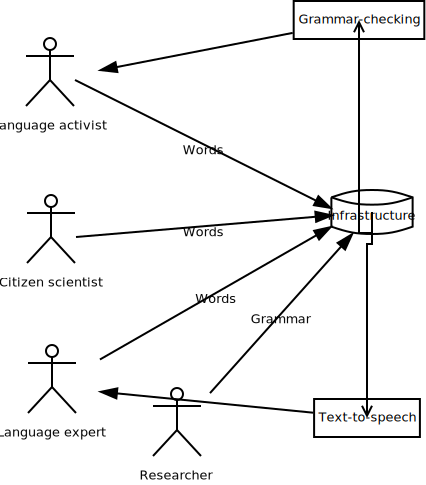
\includegraphics[width=.9\textwidth]{infra-diagram}
    \caption{Ideal workflow for infrastructure in NLP apps
    (simplified; in reality there is a fully connected graph of dozens of apps and stakeholders)
    \label{fig:infra}}
\end{figure}

One of the core values that makes this all possible is based on the \textit{free/libre open source software} (FLOSS)  movement, which in way is turning into free science and open data movements in the academia.
In the old times of single scientists keeping their word-lists and grammar sketches in the desk drawers, eventually  to  be  published  in  a  grand  tome  with  a  high  price  and  restricting licence schemes, it was not easily possible for other researchers and the language community at large to start contributing and further developing the resources.
However, the free and open source movement has already enabled such huge projects like Wikipedia, a massive crowd-sourced online encyclopedia made by humans, and this work is in a way trying to harness the same approaches in the field of linguistics and lexicography.

One of the recent innovations in software engineering is the concept of \textit{Continuous Deployment} and \textit{Continuous Integration} (CD/CI).
This means that a software is developed all the time and the updates are made public immediately, and there is an automatic infrastructure to test the software quality and send the end-users updated versions.
This translates directly to work with language resources; when language users discover a word is not supported by the spell-checker or similar NLP software they can submit it to the infrastructure and get an updated version of the software with the word included within hours instead of after months of development cycle.
In this article we study the implementation of such CI/CD infrastructures within the NLP systems.

\subsection{Prior Art}

The  role of computational linguistics infrastructures in projects for cooperating with citizen scientists and language experts to create NLP software has not been very extensively studied.
Some existing work has been published on the topic of co-operation of linguists and engineers in large scale infra-structure like projects, e.g.~\cite{moshagen2014open,bird2001formal,maxwell2008joint,scannell:2006}.
In the part of involving the audience more in the infra-structure usage some recent projects have built on the existing and documented infrastructures, such as~\cite{alnajjar-etal-2020-verdd,rueter-hamalainen-2017-synchronized}
The other part of infrastructure usage and uptake is documented as outreach activities, for such relevant is also software projects, like UralicNLP~\cite{Hämäläinen2019}\footnote{\url{https://github.com/mikahama/UralicNLP/}}, and activities of education networks like COPIUS\footnote{\url{https://www.copius.eu/index.php}} and labs like FU-Lab.\footnote{\url{https://fu-lab.ru/}}

\section{Infrastructures and Resources} \label{sec:unfra}

In this article we survey some of the main free/open source repositories for Uralic NLP specifically related to lexicography and morphology.
The main goal of much of our work is to release NLP-based tools for end-users, be it machine translation or spell-checking and correction, and the lexicography and contributions linguistic research are achieved as a side effect.
As one of the goals of the infrastructures is to lower the barrier to entry, we put an emphasis in this article to the infrastructure frameworks built to make it easier and more accessible.
In table~\ref{table:infra} we show an overview of the languages and resources for our infrastructures: GiellaLT and Apertium and for comparison other FLOSS infrastructures: CommonVoice\footnote{\url{https://commonvoice.mozilla.org}} and Universal Dependencies\footnote{\url{https://universaldependencies.org}} and UniMorph\footnote{\url{https://github.com/unimorph/}}.


\begin{table}
\centering
\caption{Infrastructures and the languages and resources they have.\label{table:infra}}
\begin{tabular}{lrl}
\toprule
\textbf{Infra - stuff} & \textbf{Languages} & \textbf{NLP resources} \\
\midrule
GiellaLT &  121 & Morphological analysis\\
         &      & Text-To-Speech \\
         &      & Spell and Grammar-checking \\
Apertium &  181 & Morphological analysis \\
         &  237 & Machine translation \\
\midrule
Common Voice & 78 & Speech recognition \\
            &    & Speech synthesis \\
Universal Dependencies & 104 & Treebanking \\
  & & Dependency Grammar \\
Unimorph & 122 & Example \\
 & & word-forms \\
\bottomrule
\end{tabular}
\end{table}

One important feature of a language technology infrastructure is separation of the technology and data.
This means that the language experts can collect and curate data, while the engineers improve and add NLP systems, and when a new or improved system for a specific NLP application is finalised, it can be applied to all languages providing language data in the infrastructure.
In practice for example, this has in past meant, that when new research was published making weighted finite-state spell-checking and correction end-user usable~\cite{pirinen2014state}, all languages in the infrastructure could have an additional (albeit basic) spell-checker and corrector.
Both in GiellaLT infra and Apertium system this is implemented at low level by simply applying the necessary changes to all of the language repositories.
Due to potential of complicated interactions and change conflicts in this phase, both infrastructures have built additional tooling to ease the process: gut\footnote{\url{https://github.com/divvun/gut/}} and Apertium-init\footnote{\url{https://github.com/Apertium/Apertium-init/}}
In the core both systems are based on partial templating, with main difference being in the implementation technology: Rust and Python respectively.

\subsection{Testing}

One feature that an infrastructure is useful for as a supporting role for citizen science and crowdsourcing lexicography is quality assurance.
In the NLP software this is done by automated testing.
The automated tests for an end-user facing software can vary from as simple unit and integration testing as ensuring that you can enter word-forms and get analyses or translations back to as intricate as ensuring that the translation or spell-checking quality does not decrease.
The testing methodology follows from software engineering and tends to use the same terminology: Unit testing, regression testing, integration testing and so forth.
One of the testing approaches many linguists might be most acquainted with is a form of regression testing \cite{bender2007validation}.
One of the recent developments in software engineering is automated testing of each commit on the server, using \textit{continuous integration}.
Continuous integration is set up to ensure that no changes to the lexicon are breaking the system or decreasing the results.

There are two problems that arise with complex NLP systems and automated testing: firstly, a full coverage testing on substantial material can take much more time and processing resources than is available on a freely available CI services.
Secondly, complex NLP systems do not only break from changes within the local lexicographical data, but also from other parts of infrastructure changing.
With the theme of rule-based machine translation this is obvious: each project depends at least from three different lexicographical projects: the \textit{source} language dictionary, the \textit{target} language dictionary and the \textit{bilingual} dictionary, and change in any of these can throw the translation off.
For other NLP pipelines, similar problems arise from changes in the build infrastructure, for example handling of capitalisation, tokenisation and even tagging standard changes.
The first problem of limited processing power we have partially solved with self-hosted and customised build servers, however, this does introduce a non-standard non-trivial component to the mix so it is unoptimal for the purpose of this article (not easily reproducible).
The second problem still exists in our build systems, however we are researching on potential solutions.


\subsection{Deploying}

One feature that infrastructure provides to scientists and language experts is turning their  lexicons and grammars into end-user products fro the whole language community: for example languages  in GiellaLT and Apertium repository are provided to users of LibreOffice, or Linux-based systems as packages for spell-checking and correction~\cite{pirinen2014state}.\footnote{\url{https://divvun.org}}

The most common approach for deployment is, is to simply provide a standard build system, such as auto-tools based one, and have the distributors of systems pick it up for their users; this has been the traditional approach especially within the Linux ecosystem and other free / open systems.
This is not always feasible option for minority language technology, e.g. due to lack of interest and necessary expertise on behalf of the distribution providers, for other approaches we have build custom repositories\footnote{\url{https://Apertium.projectjj.com/apt/}}, and supplementary parts to packaging systems\footnote{\url{http://pahkat.uit.no/}}, which, while not ideal for average end users, are good enough to get the software to a majority of the end users.

\subsection{Documentation}

One of our goals in the original infrastructure designs has been to introduce the concept of \textit{Literate Programming}~\cite{knuth1984literate} into NLP.
The idea of producing documentation, even books, from well-commented source code is well within reach or natural language processing, lexicographical databases and grammar rules are typically the main meal of linguistic literature in general.
For example in Fennistic tradition, it is not untypical to see a grammar book formatted in form of dozens and dozens of examples listed or tabulated accompanying every description of every grammatical phenomenon, this is very near to rule-based NLP format already.
The current implementation of the literate programming scheme in giellaLT infra follows the light-weight literate programming style most programming languages have eventually adopted as well, namely \textit{doc comments}.
What this means is we have specially formatted comment blocks within source code, that can be, together with context-relevant code, be re-used as documentation, as well as \textit{unit tests}.
Compare this to Python's docstrings\footnote{\url{https://www.python.org/dev/peps/pep-0257/}} and doctests\footnote{\url{https://docs.python.org/3/library/doctest.html}}.
It is noteworthy, that mostly, in lexicography and grammar, tests, are nothing more than example word forms and their preferred annotations, be it grammatical analysis or perhaps spelling corrections, this, naturally, is in and of itself interesting for a linguist even without the testing feature.
As a recent feature for the documentation comments, the output format has been updated to GitHub's github-pages format and a prototypical examples can be found at the time of writing in the GiellaLT github space\footnote{\url{https://giellalt.github.io}, see for example \url{https://giellalt.github.io/lang-fin/fin.html}}.


\section{Discussion and conclusions} \label{sec:discussion}

We have built various infrastructures for enabling various groups of contributors to contribute linguistic data.
Currently our infrastructures are used to involve large number of researchers in providing digital language tools for large number of marginalised languages.

In the table~\ref{table:infra} we give the amount of languages being worked on within the infrastructures, while the numbers do not directly tell of the quality, there are further ways of determining how much the languages have been worked on in each of the systems.
Within GiellaLT and Apertium communities we have opted for self-classifying the production quality of the languages as such: in GiellaLT registry\footnote{\url{https://github.com/divvun/registry\#languages}} at the time of writing we find  8 full \textit{production} quality and 27 \textit{beta} testing phase languages (out of 128), in Apertium correspondingly 53 \textit{trunk} translators and 39 \textit{nursery} translators (out of 237).\footnote{at the time of writing, this can obviously change fast in a fast-moving user community}
The repositories Common Voice, Universal Dependencies and Unimorph on the other hand do not include classifications, but we can study them rather by comparing the sizes: the biggest recording size in English is 1800 hours, and 36 have 10 or more hours of confirmed recordings, out of the 78.
For Universal Dependencies biggest data set is German with 3.753 million dependency trees, with 43 having over 100 thousand trees.
In unimorph, Finnish is the biggest dataset with over 2 million word-forms, with 27 languages containing over 100 thousand word forms.

%% From template: equations theorems proofs

%% \begin{equation}
%% x + y = z
%% \end{equation}


%% \begin{theorem}
%% This is a sample theorem. The run-in heading is set in bold, while
%% the following text appears in italics. Definitions, lemmas,
%% propositions, and corollaries are styled the same way.
%% \end{theorem}

%% \begin{proof}
%% Proofs, examples, and remarks have the initial word in italics,
%% while the following text appears in normal font.
%% \end{proof}

%\section{Conclusion} \label{sec:conclusion}

We have two infrastructures for NLP systems that have provided people with various tools and software for years.
They have also improved continuously and still actively used.

\section*{Acknowledgments}

Building and using infrastructures takes a large developer base and the authors of the article are just a small part of these communities.
Thanks goes to everyone at GiellaLT\footnote{\url{https://github.com/orgs/giellalt/people}}, Divvun\footnote{\url{https://github.com/orgs/divvun/people}}, and Apertium\footnote{\url{https://github.com/orgs/Apertium/people}} communities.

\bibliographystyle{splncs04}
\bibliography{mybibliography}

\end{document}
